\section{Results}

\subsection{Evaluation Data and the Completeness Filter}

We evaluate on the MNIST test set \cite{lecun1998}, 10,000 handwritten digit
images rendered at 100$\times$100 pixels. The completeness filter is a per-image
annotation made by hand before any classification run and recorded in
\texttt{mnist\_all\_manifest.csv} in the public repository: an image is marked
complete when its stroke has no break and incomplete otherwise. The annotation
uses only that structural property, not the class label and not the
classifier's output. A broken stroke
violates the assumption the graph representation of Section~III rests on, and
the graph built from such an image describes a different figure. Recognising
broken structures needs a separate mechanism, associative recognition, which
the system does not implement.

The filter admits 8,707 of the 10,000 test images and excludes 1,293, or
12.9\%. The accuracy reported below is therefore conditional on the filter
and does not transfer to full MNIST. The filter also acts unevenly across
classes (Table~\ref{tab:perclass}). Class~1 keeps 1,129 of its 1,135 test
images (99.5\%), while class~8 keeps 582 of 974 (59.8\%). Per-class figures
therefore rest on samples of very different size, and class~8 has the narrowest
basis.

A further 22 admitted images (0.25\%) failed graph construction:
skeletonization produced no connected graph at any threshold of the retry
ladder (Section III-B). We count these as pipeline
errors. A classification decision was produced for 8,685 images.

\subsection{Classification Results}

On the 8,685 classified images the system reaches 91.13\% accuracy,
91.92\% precision, 91.13\% recall and 91.34\% F1. The three averaged
figures are weighted by class support; the unweighted macro averages over the
ten classes are 92.22\%, 91.22\% and 91.54\%.

\begin{table}[t]
\caption{Per-class evaluation. ``Admitted'' is the count passing the
completeness filter and ``share'' its fraction of that class in the MNIST test
set. ``Classified'' is the count that produced a classification decision;
precision, recall and F1 are computed on that column and the totals are
support-weighted.}
\label{tab:perclass}
\centering
\footnotesize
\setlength{\tabcolsep}{3pt}
\begin{tabular}{lrrrrrr}
\toprule
Class & Admitted & Classified & Share, \% & Prec., \% & Recall, \% & F1, \% \\
\midrule
0     & 830   & 830   & 84.7 & 99.87 & 91.93 & 95.73 \\
1     & 1,129 & 1,122 & 99.5 & 93.69 & 96.52 & 95.08 \\
2     & 956   & 955   & 92.6 & 92.28 & 77.59 & 84.30 \\
3     & 969   & 968   & 95.9 & 91.78 & 95.76 & 93.73 \\
4     & 953   & 950   & 97.0 & 92.15 & 84.00 & 87.89 \\
5     & 796   & 796   & 89.2 & 93.97 & 91.96 & 92.95 \\
6     & 742   & 741   & 77.5 & 84.88 & 92.44 & 88.50 \\
7     & 1,014 & 1,011 & 98.6 & 82.01 & 95.15 & 88.10 \\
8     & 582   & 581   & 59.8 & 98.74 & 94.49 & 96.57 \\
9     & 736   & 731   & 72.9 & 92.85 & 92.34 & 92.59 \\
\midrule
Total & 8,707 & 8,685 & 87.1 & 91.92 & 91.13 & 91.34 \\
\bottomrule
\end{tabular}
\end{table}

Per-class figures spread much wider than the totals
(Table~\ref{tab:perclass}). Precision is highest for class~0 (99.87\%) and
class~8 (98.74\%), whose concepts attract almost nothing from other classes.
Precision is lowest for class~7 (82.01\%) and class~6 (84.88\%), which take
on images belonging to neighbouring classes. Recall orders the classes
differently, with class~2 (77.59\%) and class~4 (84.00\%) at the bottom.

The system made 770 wrong decisions: 726 assigned the image to a wrong class,
and in 44 no concept activated and the image was left unrecognised, mostly in
class~6 (16) and class~8 (14).

\begin{figure}[t]
\centering
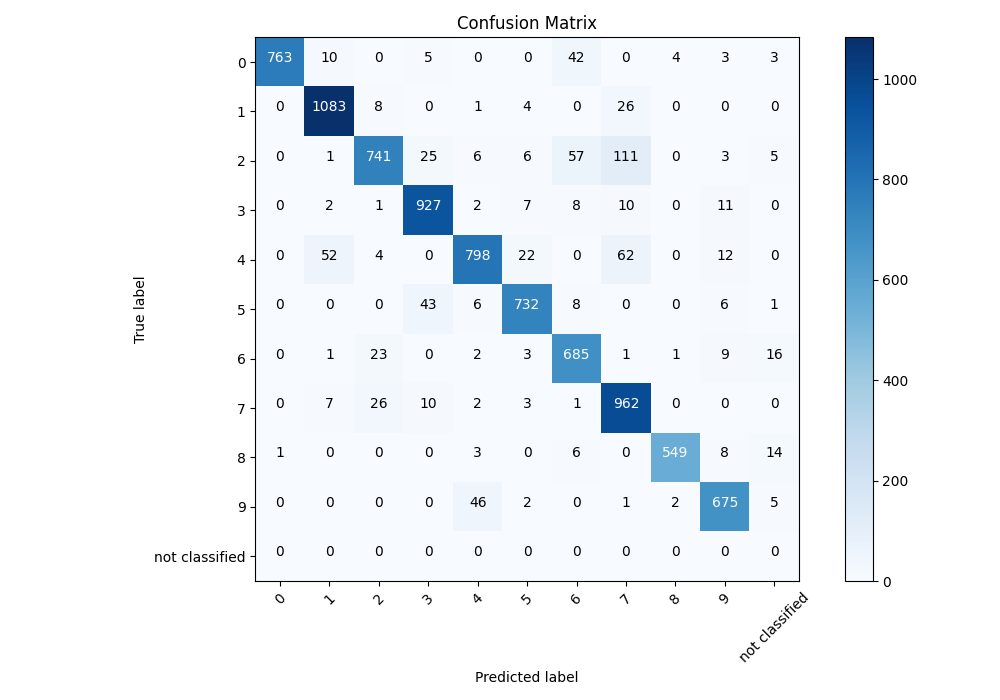
\includegraphics[width=\columnwidth,trim=96 13 60 27,clip]{figures/fig_confusion.png}
\caption{Confusion matrix over the 8,685 classified images, taken from the run
artefacts. Rows are true classes, columns predicted classes; the last column
holds images that activated no concept, and the last row is empty by
construction.}
\label{fig:confusion}
\end{figure}

Errors concentrate on a few pairs (Fig.~\ref{fig:confusion}). Written as true
class $\rightarrow$ predicted class, the most frequent pairs are
2$\rightarrow$7 with 111 cases, 4$\rightarrow$7 with 62, 2$\rightarrow$6 with
57, 4$\rightarrow$1 with 52, 9$\rightarrow$4 with 46, 5$\rightarrow$3 with 43,
0$\rightarrow$6 with 42, 1$\rightarrow$7 with 26, 7$\rightarrow$2 with 26, and
2$\rightarrow$3 with 25. These ten pairs cover 490 of the 726 wrong-class
assignments, or 67.5\%. Two classes produce nearly half of all errors:
class~2 with 214 and class~4 with 152.

\subsection{Decision Trace}

Every decision decomposes into values a reader can check. We show this on
image \cid{mnist\_test\_2\_00766}, true class 2, predicted 7. We chose a
misclassification: an explanation has to hold for a wrong decision as well
as for a correct one. Fig.~\ref{fig:trace} shows the construction of the graph and the two
competing concepts; Table~\ref{tab:trace} gives the decision trace.

\begin{figure*}[t]
\centering
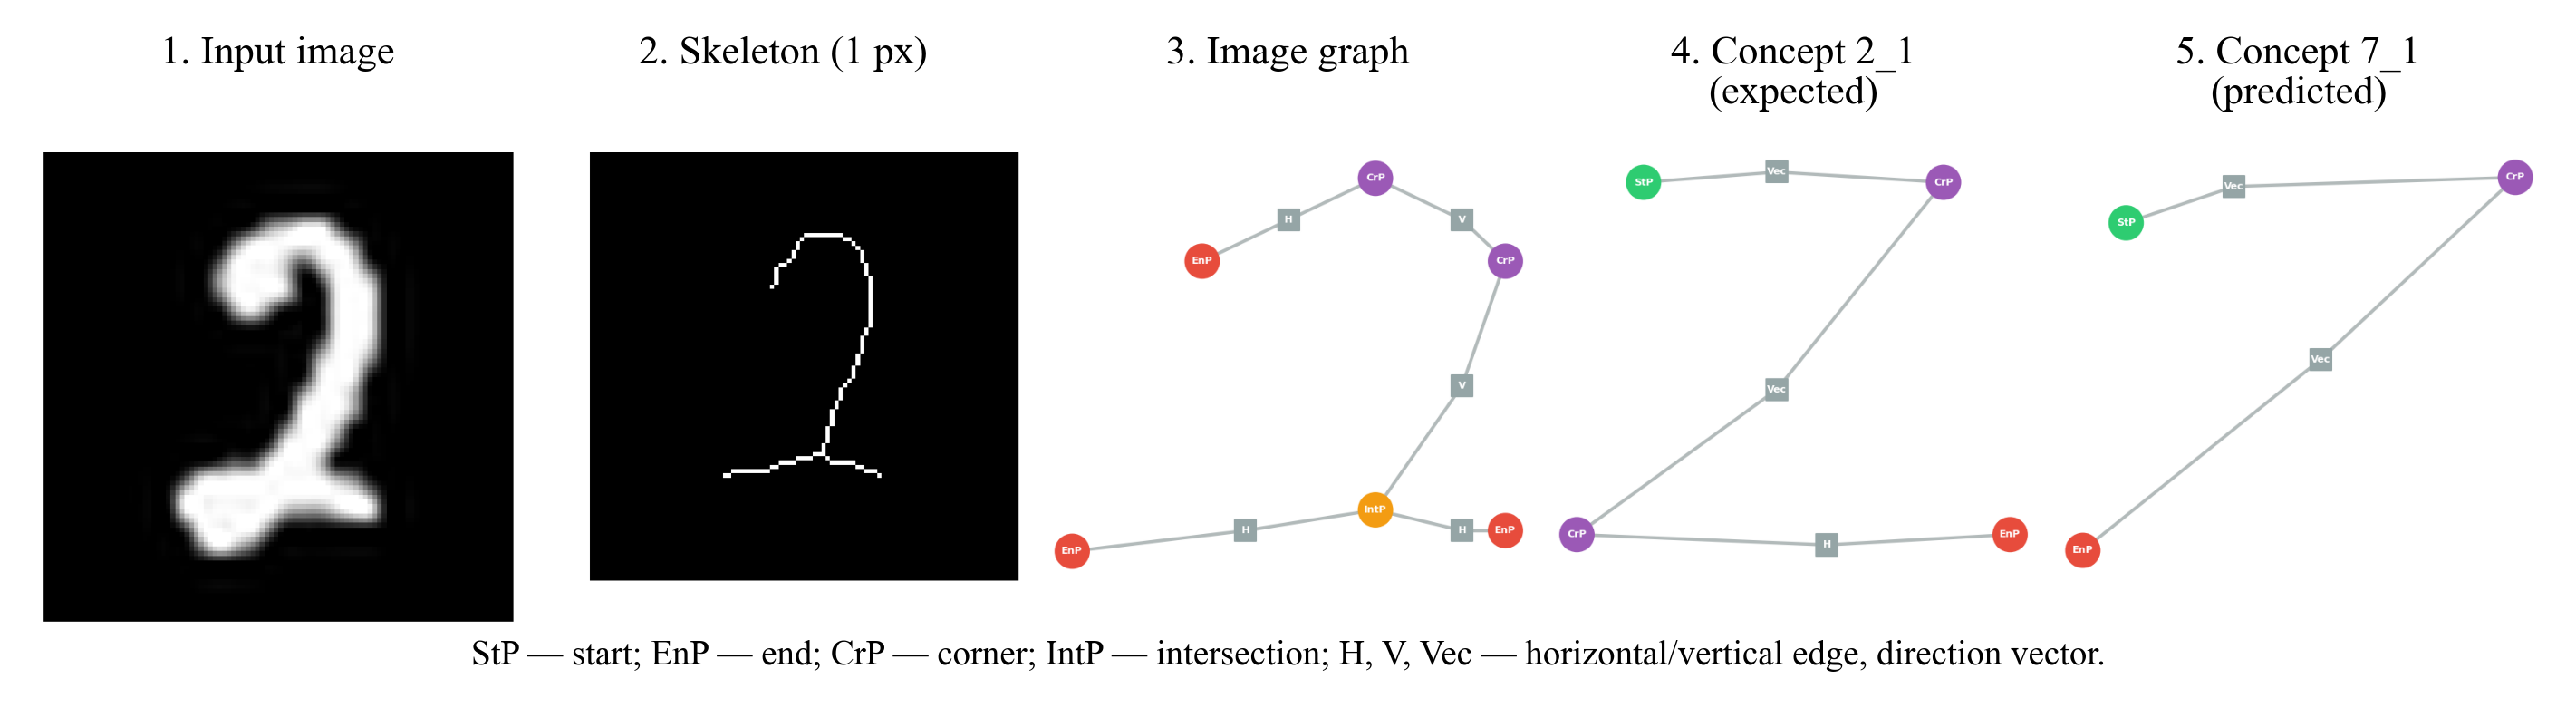
\includegraphics[width=\textwidth]{figures/fig_trace.png}
\caption{Decision trace for \cid{mnist\_test\_2\_00766}, in five panels: the
input image; the 1-pixel skeleton; the image graph with Point and Vector nodes;
concept \cid{2\_1}, expected; concept \cid{7\_1}, predicted. The lower loop of
the digit is already absent in the skeleton, so the image graph carries neither
a cycle nor an intersection point.}
\label{fig:trace}
\end{figure*}

The image graph has complexity 21. The complexity pre-filter runs first. The
richer concept of digit~2, \cid{2\_2}, has 12 nodes and complexity 24, so the
condition $24 > 21$ removes it before any comparison. The impoverished input is
visible in the image: binarization lost the lower loop of the 2, the closed
structure became an open spur, and the graph holds neither a cycle nor an
intersection point.

Two concepts then compete. Concept \cid{7\_1} has five nodes, every one of them
substituted within the learned intervals of the concept, at substitution costs
between 0.04 and 0.39, and reaches similarity 0.8317. Concept \cid{2\_1} has
seven nodes and matches the input structurally, but three of its nodes each
carry one feature outside its interval, and each takes the full 1.0 penalty:
the StartPoint on \texttt{distance\_to\_centroid} (0.56 against $[0.69, 1.00]$),
a CornerPoint on \texttt{normalized\_x} (0.20 against $[-0.70, 0.10]$) and a
horizontal Vector node on \texttt{length\_ratio\_to\_max} (0.31 against
$[0.43, 1.00]$). With their in-range features added, the three node
substitution costs are 1.01, 1.10 and 1.30. Its similarity is 0.7300.

Complexity is $\kappa = 9$ for \cid{7\_1} and $\kappa = 13$ for \cid{2\_1}, so
the prior of \eqref{eq:score} favours \cid{2\_1} by 0.053 and does not close
the gap. Winner-take-all on the score picks \cid{7\_1}: 1.149 against 1.100.

\begin{table}[t]
\caption{Decision trace for \cid{mnist\_test\_2\_00766}.}
\label{tab:trace}
\centering
\footnotesize
\setlength{\tabcolsep}{3pt}
\begin{tabular}{lrrp{3.0cm}rr}
\toprule
Concept & Nodes & $\kappa$ & Matching outcome & Sim. & Score \\
\midrule
\cid{2\_2} & 12 & 24 & removed by the pre-filter, $24 > 21$ & --- & --- \\
\cid{7\_1} & 5 & 9 & all five nodes substituted inside the intervals, costs
0.04--0.39 & 0.8317 & 1.149 \\
\cid{2\_1} & 7 & 13 & three nodes with one out-of-range feature each; node costs
1.01 / 1.10 / 1.30 & 0.7300 & 1.100 \\
\bottomrule
\end{tabular}
\end{table}

The mechanism holds beyond this one image. Across all 111 2$\rightarrow$7
errors, \cid{2\_1} entered the comparison every time and lost on similarity
every time, by a mean margin of 0.14. In none of the 111 cases did a concept of
digit~2 win on similarity and then lose after the complexity prior was applied.

\subsection{Inference Cost}

An image is compared against at most 13 concepts, each comparison under a
5\,s deadline, so the theoretical upper bound is 65\,s per image. The measured
stage times stay far below it.

The pipeline ran on a single workstation in 24 Docker containers: four
skeletonization instances, four contour analysis instances and sixteen
classification instances. Per-stage medians come from the profiling records:
skeletonization 52.8\,ms with a maximum of 533\,ms, contour analysis
211.5\,ms with a maximum of 1,905\,ms, and the classification stage, meaning
all GED comparisons for one image together, 167.1\,ms with a 99th percentile of
about 0.84\,s and a maximum of 1,414\,ms. No profiled image came close to the
5\,s deadline of a single comparison. On the profiled images the solver
therefore finished its search before the deadline, and the reported distances
are completed results, not deadline-truncated ones.

One caveat limits the use of these medians. Profiling records exist only for
the 770 misclassified images, so the profiled subset is biased and
correctly classified images are absent from it. The available data does not fix
the direction of the bias. The number of GED comparisons per image is set by
the complexity pre-filter, not by the correctness of the final decision. The medians are therefore not a typical-case estimate.
The run does not record its own total duration, and the system does not store
the time of an individual GED comparison.

\section{Discussion}

The explanation here is the decision object itself. No second model
approximates the classifier from outside. To see why an image received a class,
a reader opens the image graph and reads the learned intervals of the winning
concept attractor and the cost charged for each feature. The trace in
Section~IV-C runs the whole chain, from the complexity pre-filter down to one
out-of-range value, \texttt{normalized\_x} at 0.20 against the interval
$[-0.70, 0.10]$. Post-hoc attribution methods build
their explanation after the fact by perturbing the input
\cite{ribeiro2016,lundberg2017}, and that construction can be manipulated
\cite{slack2020}. Decisions with consequences are better taken by models
interpretable by construction \cite{rudin2019}.

The same property applies to the failures. Binarization loses the lower loop of
the digit, so the image graph carries no intersection point, and the pre-filter
removes \cid{2\_2} in 86 of the 111 2$\rightarrow$7 cases. The pre-filter is
not the cause: in a control run with it lifted, \cid{2\_2} won none of the 111,
because an intersection-point condition blocks its match to a graph without an
intersection. The error has two causes: the lower loop lost at binarization,
and the full interval penalties on \cid{2\_1} against the in-interval match of
the five-node \cid{7\_1}. The error can be named and its prevalence checked
over all 111 cases.

Traceability defines the application niche: tasks where the answer has to be
auditable. Verification of handwritten marks in document workflows, inspection
of industrial marking, and tutoring systems that must show a learner the reason
for a grade share the property that a human resolves every disputed decision. A
decision record of the named concept, its node substitutions and its
per-feature costs goes into that review without a separate explanation module.
For a dependability audience the property on offer is auditability: every
decision leaves a record that a person can check against the input without
re-running the system.
The small training set also lowers the cost of starting on a new set of marks:
one concept attractor forms from 3--9 samples and their augmented variants
(Section III-D). An earlier
prototype reported 82.44\% on six classes \cite{parzhyn2025energy}; the two
numbers are not comparable, since the class set, the test set size and the
formation procedure all differ.

Several limitations bound the result. The headline metric is conditional on the
completeness filter, which excludes 12.9\% of the test set unevenly across
classes. The inference cost is measured, but the profiled subset holds only
misclassified images, and per-comparison timing does not exist. The 76 training
samples were selected by hand and the sensitivity of accuracy to that selection
was not measured, so part of the accuracy may come from a fortunate choice. The
training samples were chosen on the same completeness criterion as the test
filter, so the evaluation measures the system inside the regime it was built
for, and the exclusion does the most work in the classes with the lowest
admission rates (8, 9 and 6). Sensitivity of a concept attractor to the
order of its samples was not measured in this study. Tolerance to rotation is
limited to the small range covered by augmentation. The contour representation
discards texture and gradients, which confines the method to silhouette and
stroke images. Broken contours need associative
recognition, which the system does not have.

\section{Conclusion}

We formed an alphabet of 13 concept attractors for ten digit classes by
structural reduction of 76 hand-selected training samples and their augmented
variants, with no backpropagation anywhere in the procedure. Classification by graph edit
distance with interval-based feature weighting recognises 8,685
complete-contour MNIST images at 91.13\% accuracy, 91.92\% precision,
91.13\% recall and 91.34\% F1. The evaluation is stated with its filter:
12.9\% of the test set is excluded and the metric does not carry over to
full MNIST. Each decision decomposes into a named concept, a list of
node substitutions and a per-feature cost, and the dominant 2$\rightarrow$7
error was traced through that decomposition over all 111 cases. Inference cost
was measured per pipeline stage, and on the profiled images the 5\,s deadline of a
single comparison was not reached. Work ahead covers associative recognition for broken
contours, per-comparison timing on the full test set, and a sensitivity study
of the training sample choice. The source code and the run artefacts are public
at \url{https://github.com/kbokh/NaturalAGI}.
